\documentclass[]{book}\usepackage{knitr}

%%%%%%%%%%%%%%%%%%%%%%%%%%%%%%%%%%%%%%
% packages
%%%%%%%%%%%%%%%%%%%%%%%%%%%%%%%%%%%%%%
\usepackage[margin=1in]{geometry}
\usepackage[T1]{fontenc}
\usepackage{amsmath,dsfont}
\usepackage{caption}
\usepackage{floatrow}
% \usepackage[maxbibnames=99, backend=biber, giveninits=true, natbib=true, uniquename=init, style=apa]{biblatex}
% \DeclareLanguageMapping{english}{english-apa}

%\renewcommand{\baselinestretch}{1.5} % line spacing (for the journal) 
\usepackage[utf8]{inputenc}
\usepackage{bm}
\usepackage{verbatim}
\usepackage{float}
\usepackage{mwe}
\usepackage{color,soul}
\usepackage{threeparttable}
\usepackage{graphicx}
\usepackage{subcaption}
\usepackage{mwe}
\usepackage{mdframed}
\usepackage{xcolor}
\usepackage{bbm}
%\usepackage{authblk}

\usepackage{hyperref}
% References
\usepackage[
backend=bibtex,
style=authoryear,
sorting=ynt,
natbib=true
]{biblatex}
% \renewcommand{\citet}[#1]{\textcite{#1}}
%\usepackage{natbib}
%\bibliographystyle{apalike}
%\bibpunct[, ]{(}{)}{,}{a}{}{,}%
%\def\bibfont{\small}%
%\def\bibsep{\smallskipamount}%
%\def\bibhang{24pt}%
%\def\newblock{\ }%
%\def\BIBand{and}%

%\soulregister\cite7
%\soulregister\ref7
%\soulregister\eqref7
%\soulregister\pageref7
%\soulregister\equation7

\usepackage{multirow}
\usepackage{makecell}
\usepackage{booktabs}
\usepackage{array}
\usepackage{hhline}
\renewcommand\theadalign{bc}
\renewcommand\theadfont{\bfseries}
\renewcommand\theadgape{\Gape[4pt]}
\renewcommand\cellgape{\Gape[4pt]}
\usepackage{lscape}
\usepackage{mathtools}
\usepackage{bbm}
\usepackage{romanbar}
\usepackage{amsthm}
\usepackage{enumerate}
\usepackage{rotating}
\usepackage{tikz}
\usetikzlibrary{matrix}
\usetikzlibrary{calc,intersections}
\usepackage{mathrsfs}

%%%%
\usepackage{color}
\newcommand{\colr}[1]{{\color{red} {#1}}}
\newcommand{\colb}[1]{{\color{blue} {#1}}}
%%%%%%%%%%%%%%%%%%%%%%%%%%%%%%%%%%%%%%
% definitions
%%%%%%%%%%%%%%%%%%%%%%%%%%%%%%%%%%%%%%
\newtheorem{theorem}{Theorem}[section]
\newtheorem{corollary}[theorem]{Corollary}
\newtheorem{lemma}[theorem]{Lemma}
\newtheorem{proposition}[theorem]{Proposition}

% Definitions  etc.
\theoremstyle{definition}
\newtheorem{definition}[theorem]{Definition}
\newtheorem{example}{Example}[section]
\theoremstyle{remark}
\newtheorem{remark}[theorem]{Remark}
\newtheorem{observation}[theorem]{Observation}

%%%%%%%%%%%%%%%%%%%%%%%%%%%%%%%%%%%%%%
% Math commands
%%%%%%%%%%%%%%%%%%%%%%%%%%%%%%%%%%%%%%
\newcommand{\bol}[1]{\mbox{\boldmath$#1$}}
\newcommand{\mb}[1]{\mathbf{#1}}
\newcommand{\eqdist}{\stackrel{d}{=}}
\newcommand{\bSigma}{\mathbf{\Sigma}}
\newcommand{\hbSigma}{\hat{\bol{\Sigma}}}
\newcommand{\bDelta}{\bol{\Delta}}
\newcommand{\hw}{\hat{w}}
\newcommand{\bmu}{\bol{\mu}}
\newcommand{\hbmu}{\hat{\bol{\mu}}}
\newcommand{\tbmu}{\tilde{\bol{\mu}}}
\newcommand{\bet}{\bol{\eta}}
\newcommand{\btheta}{\bol{\theta}}
\newcommand{\bb}{\mathbf{b}}
\newcommand{\hbb}{\mathbf{\hat{b}}}
\newcommand{\bx}{\mathbf{x}}
\newcommand{\bxb}{\bar{\mathbf{x}}}
\newcommand{\bQ}{\mathbf{Q}}
\newcommand{\hbQ}{\hat{\mathbf{Q}}}
\newcommand{\be}{\mathbf{e}}
\newcommand{\by}{\mathbf{y}}
\newcommand{\byb}{\bar{\mathbf{y}}}
\newcommand{\tby}{\tilde{\mathbf{y}}}
\newcommand{\bt}{\mathbf{t}}
\newcommand{\bC}{\mathbf{C}}
\newcommand{\bP}{\mathbf{P}}
\newcommand{\bM}{\mathbf{M}}
\newcommand{\bH}{\mathbf{H}}
\newcommand{\bL}{\mathbf{L}}
\newcommand{\bl}{\mathbf{l}}
\newcommand{\br}{\mathbf{r}}
\newcommand{\hbm}{\bol{\hat{\mu}}}
\newcommand{\hbet}{\bol{\hat{\eta}}}
\newcommand{\bhR}{\hat{\mathbf{R}}}
\newcommand{\bhA}{\hat{\mathbf{A}}^{-1}}
\newcommand{\bR}{\mathbf{R}}
\newcommand{\btR}{\mathbf{\tilde{R}}}
\newcommand{\bz}{\mathbf{z}}
\newcommand{\bd}{\mathbf{d}}
\newcommand{\bB}{\mathbf{B}}
\newcommand{\bE}{\mathbf{E}}
\newcommand{\bX}{\mathbf{X}}
\newcommand{\bY}{\mathbf{Y}}
\newcommand{\bv}{\mathbf{v}}
\newcommand{\bw}{\mathbf{w}}
\newcommand{\hbw}{\mathbf{\hat{w}}}
\newcommand{\btL}{\mathbf{\tilde{L}}}
\newcommand{\bOne}{\mathbf{1}}
\newcommand{\bzero}{\mathbf{0}}
\newcommand{\bI}{\mathbf{I}}
\newcommand{\xp}{\mbox{exp}}
\newcommand{\tr}{\operatorname{tr}}
\newcommand{\Cov}{\mbox{Cov}}
\newcommand{\E}{\mbox{E}}
\newcommand{\Var}{\mbox{Var}}
\newcommand{\ve}{\mbox{vec}}
\newcommand{\tbx}{\tilde{\bx}}
\newcommand{\bA}{\bol{A}}
\newcommand{\ba}{\bol{a}}
\newcommand{\brx}{\breve{\bx}}
\newcommand{\brm}{\breve{\bol{\mu}}}
\newcommand{\brA}{\breve{\bA}}
\newcommand{\si}{\boldsymbol{\sigma}}
\newcommand{\tbF}{\tilde{\mathbf{\Phi}}}
\newcommand{\bF}{\mathbf{F}}
\newcommand{\bn}{\boldsymbol{\nu}}
\newcommand{\byy}{\bn_y}
\newcommand{\bxi}{\boldsymbol{\xi}}
\newcommand{\bD}{\mathbf{D}}
\newcommand{\eps}{\pmb{\varepsilon}}
\newcommand{\bW}{\mathbf{W}}
\newcommand{\bV}{\mathbf{V}}
\newcommand{\bla}{\boldsymbol{\lambda}}
\newcommand{\bry}{\breve{\by}}
\newcommand{\tbw}{\tilde{\bw}}
\newcommand{\tbSigma}{\tilde{\bSigma}}
\newcommand{\bO}{\mathbf{O}}
\newcommand{\brn}{\breve{\bn}}
\newcommand{\bOmega}{\boldsymbol{\Omega}}
\newcommand{\bomega}{\boldsymbol{\omega}}
\newcommand{\tbn}{\tilde{\bn}}
\newcommand{\tbB}{\tilde{\bB}}
\newcommand{\tbb}{\tilde{\mathbf{b}}}
\newcommand{\bS}{\mathbf{S}}
\newcommand{\sx}{\bar{\mathbf{x}}}
\newcommand{\sy}{\bar{\mathbf{y}}}
\newcommand{\Tr}{\text{tr}}
\newcommand{\bG}{\mathbf{G}}
\newcommand{\bu}{\mathbf{u}}
\newcommand{\bU}{\mathbf{U}}
\newcommand{\bTheta}{\mathbf{\Theta}}
\newcommand{\ta}{\alpha}
\newcommand{\tb}{\beta}
\newcommand{\bZ}{\mathbf{Z}}
\newcommand{\bT}{\mathbf{T}}
\newcommand{\bq}{\mathbf{q}}
% \newcommand{\bt}{\mathbf{t}}
\newcommand{\hbtheta}{\bol{\hat{\theta}}}
\newcommand{\ones}{\mathbf{1} }
\newcommand{\bgamma}{ \boldsymbol{\gamma} }
\newcommand{\bGamma}{ \boldsymbol{\Gamma} }
\newcommand{\optn}[1]{\operatorname{#1}}
\newcommand{\VaR}{\operatorname{VaR}}
\newcommand{\CVaR}{\operatorname{CVaR}}
\newcommand{\prob}{\mathsf{P}}
\newcommand{\real}{\mathbb{R}}
\newcommand{\Kappa}{\mathrm{K}}
\newcommand{\argmin}{\mathop{\mathrm{argmin}}}

% Portfolio characteristics
\newcommand{\hV}{\hat{V}_{GMV}}
\newcommand{\hR}{\hat{R}_{GMV}}
\newcommand{\R}{R_{GMV}}
\newcommand{\V}{V_{GMV}}
\newcommand{\hs}{\hat{s}}

\providecommand{\keywords}[1]
{
\small	
\textbf{\textit{Keywords}:} #1
}

\renewcommand \thesubsubsection{\roman{subsubsection}.\roman{subsubsection}}


\DeclareNewFloatType{chunk}{placement=H, fileext=chk, name=}
\captionsetup{options=chunk}
\renewcommand{\thechunk}{Chunk~\thesection.\arabic{chunk}}
\makeatletter
\@addtoreset{chunk}{section}
\makeatother

%opening
\title{Optimal portfolios in higher dimensions - estimation and uncertainty}
\author{Erik Thorsén}
\IfFileExists{upquote.sty}{\usepackage{upquote}}{}
\begin{document}

% \SweaveOpts{concordance=TRUE}


\maketitle

\section*{Acknowledgements}

\newpage
\section*{List of papers}



\tableofcontents
%%%%%% ------------------------------------------------------------------------
\chapter[Introduction]{Introduction - making decisions and allocations}\label{ch:intro}
%%%%%% ------------------------------------------------------------------------
% General introduction to why portfolio theory and allocations are hard
% ca 1page
A portfolio is a combination of assets.
An asset might be a house, a stock, the value of a contract or any object with a price that can potentially be bought or sold.
The price of an asset develops over time.
The house prices in Stockholm, Sweden, have increased a lot in the past years\footnote{\url{https://www.maklarstatistik.se/omrade/riket/stockholms-lan/\#/villor/48m-prisutveckling}}.
However, the future price for a house is uncertain, especially given that house prices are close to all-time highs.
Will the price continue to increase or will it decrease?
If there is a change, how big will it be?
Depending on the answer, one strategy might be to sell the house today, rent something instead and buy a new house when prices have decreased.
However, to make a decision on whether or not the house should be sold today, there is a need to specify its future value. 
The future is unknown or random, in some sense.
There are many possible changes in the assets value, both in direction and magnitude.
In the context of a model there is a possibility to predict the future price through the use of historical prices.
The decision process now includes even more uncertainty.
There is uncertainty from the choice of model, the perception of past and future prices, and the uncertainty from using estimates instead of the ''true'' parameters for the model.
If the house is one asset among many then there can be as many sources of uncertainty as there are assets, if not more.
The allocation itself, in this case selling the house, is uncertain.
Uncertainty is everywhere in decisions.

The market price of a house is rarely observed.
As a matter of fact, it is only observed when it is sold.
Even though prices are rarely observed there might be houses that are similar.
There are many measurements from the same population, in this case houses which are similar to the one being sold. 
This might not be the case for the second asset that is listed above, a stock.
The frequency of which the price of a stock is observed can be much higher.
On the other hand, there is only one stock with one accompanying time series.
This makes the analysis slightly different.
There can be a lot of historical data, but no identical copies of the stock that can be used to compare and extract information from.
Prices can only be observed as they develop.

In this thesis, the aim is not to predict tomorrows price of an asset but to answer what amount of a budget should be spent on the different assets in the long run.
The methods in this thesis build upon the seminal work of \citet{markowitz1959portfolio}, what is known as Modern Portfolio Theory (MPT).
Markowitz argued that any portfolio which simply maximizes its profit will result in a naive solution.
Investing all the capital in the asset with the highest return is not sensible if the future is not known.
Such an investment will be extremely risky. 
As a consequence, Markowitz argued that any well diversified portfolio should be preferred to any non-diversified portfolio. 
A well diversified portfolio can be obtained through many different procedures.
Markowitz proposed the use of the mean and variance of the asset return distribution for the allocation problem.
If an asset has high return on average, it would make sense to invest in it if return is all that matters.
If an asset has a large variance, then it is risky to invest in this asset. 
A high return might be at the cost of a large amount of risk.
If an asset is not risky, then it would always make sense to invest in it, especially in the class of MPT portfolios this thesis studies.

%% Literature review
\section{Literature review}
%Sampling to GMV
To practically use a portfolio from the MPT framework, the parameters of the model, the mean vector and the covariance matrix, need to be estimated.
As previously mentioned, this introduces estimation uncertainty.
If the amount of data is small, then there is a large risk that the estimated portfolio will be volatile and not accurate as new data is observed.
The sampling distribution of the portfolio will have a large variance.
One important portfolio in the MPT framework is the Global Minimum Variance (GMV) portfolio.
This portfolio provides the smallest variance in the MPT framework.
\citet{okhrin2006distributional} derived the exact sampling distribution of the GMV portfolio. 
In the paper, the authors showed that the portfolio can have very fat tails depending on the sample size and the number of assets in the portfolio.
This is the first sign of a tradeof between diversification and the increasing influence of estimation uncertainty.
The portfolio has been extensively researched in many different contexts to cope with this feature.
\citet{frahm2010} extended the portfolio weights and constructed an estimator which combines the GMV portfolio with a target portfolio, much like \citet{stein1956} derived a regularization method for the sample mean vector. 
\citet{frahm2010} used properties of the sample covariance matrix to develop a regularization method for the GMV portfolio.
The method provides a way to combine the target and the GMV portfolio.
Furthermore, \citet{kempf2006estimating} showed that an estimate of the GMV portfolio can also be obtained through a regression approach.
Due to the vast literature in regression models, this approach has also spurred much research of the MPT framework (see, e.g., \citet{maillet2015global} and the references therein).

% high-dimensional
Diversification is a natural concept in MPT.
It was one of the motivations for MPT.
As more and more diversification is used, the portfolio will grow and in the most extreme case, the portfolio will contain infinitely many assets.
High-dimensional portfolios, or portfolios that contain infinite number of assets, can be thought of as a consequence of a very large amount of diversification.
Diversification is one, if not the best, risk management tool.
It should, in theory, decrease the risk of the portfolio. 
That is not always the case.
By introducing one new asset to the portfolio, more parameters than the number of assets in the portfolio need to be estimated. 
The covariance matrix suffers from the curse of dimensionality. 
In terms of estimation uncertainty, this does not scale well.
There are many ways to solve this.
\citet{lw20} and \citet{bodnar2018estimation} consider estimating high-dimensional GMV portfolios using two different approaches.
The former assumes that the eigenvectors are known and consider a nonlinear (rotational-invariant) estimation method for the covariance matrix. 
The latter develops a regularization method much like \citet{frahm2010} but does so for high-dimensional portfolios.
The mentioned papers do not assume any specific structure on the asset return distribution. 
Another common model for asset returns, which impose some structure, is the factor model (see, e.g., \cite{ross2013arbitrage}). 
A factor can be many things, such as the area in which the house is located.
\citet{ding2020high} use such a model to describe the implications of estimation to the GMV portfolio.
%\citet{golosnoy2019exponential} and \citet{cai2020high} take another approach.
%The authors of these two papers use data on a very high frequency to estimate a sequence of sample covariance matrices and use that sequence to construct high-dimensional GMV portfolios. 
The high-dimensional GMV portfolio appears in other fields as well, such as signal processing where it goes under the name beamformer (see, e.g., \cite{LiStoicaWang2004}). 

% more general MV portfolios and why GMV is most often chosen.
An argument for using the GMV portfolio in the MPT framework is that it does not depend on the mean vector.
Estimating the mean is hard (see, e.g., \citet{merton1980estimating}, \citet{best1991sensitivity}).
However, it is only one out of many portfolios in the MPT framework.
Including a target for the portfolio mean results in the mean-variance portfolio.
\citet{el2010high} investigated the weights of the mean-variance portfolio when linear constraints are introduced to the portfolio allocation problem.
This can include position restrictions as well as an investor's desire for a given return.
\citet{bodnarokhrinparolya2020} considered high-dimensional portfolios but use another portfolio allocation problem, namely the quadratic utility.
The setting is similar to \citet{bodnar2018estimation} where the authors regularize the quadratic utility portfolio towards a target portfolio in the high-dimensional setting.
\citet{karlsson2021statistical} used an extension to the quadratic utility, where a risk-free asset is introduced.
There they derived different statistical properties of its solution, known as the tangency portfolio.

The rest of this thesis is structured as follows. 
Chapter \ref{ch:MPT} presents the framework that this thesis will work within, namely MPT. 
As previously described, MPT uses information which is not available. 
It relies on parameters which are not known. 
In the subsequent chapter, Chapter \ref{ch:estim}, the models used in this thesis are introducd. 
It also introduces the more formal concept of estimation uncertainty and what it means for MPT.
Chapter \ref{ch:highdim} presents what happens in the MPT framework when an investor diviersifies as much as possible.
The portfolio will contain many, if not an infinite number, of assets.
The last two chapters, Chapter \ref{ch:papersummary} and \ref{ch:future} provide a summary of the papers presented in this thesis as well as a summary of future possible research.

All code for this thesis is available on \href{https://github.com/Ethorsn/Phd-thesis}{Github at https://github.com/Ethorsn/Phd-thesis.}

%%%%%% ------------------------------------------------------------------------
\chapter{Modern Portfolio Theory}\label{ch:MPT}
%%%%%% ------------------------------------------------------------------------


Modern Portfolio Theory was introduced by \cite{markowitz1959portfolio}. 
In his seminal work he argued that any portfolio which simply maximize its profit will result in a naive solution.
Very much like the example in Chapter \ref{ch:intro}. 
The future is unknown and (one of) the best model(s) we have for it is stochastic
Investing all your capital in the asset with the highest return is not sensible if you do not know the future.
Such an investment will cause you to take an extreme amount of risk. 
He therefore argued that any well diversified portfolio should be prefered to any non diversified portfolio. 
Such a portfolio can be obtained through many different procedures but he proposed the use of the first two moments for the allocation problem.
If an asset has high return on average, then that should be accounted for though not at the cost of large amounts of risk. If an asset implies a lot of risk, then we should try to invest small amounts in it.

We assume assets $\bx$ are random with mean $\optn{E}(\bx)=\bmu$ and covariance matrix $\optn{Var}(\bx)=\bSigma$. Although there is usually little restriction on $\bmu$ there is usually very specific restrictions on the covariance matrix $\bSigma$. Since the covariance matrix is a subject of its own we dedicate the next section to it and disregards these restrictions for now. We will merely say that it is well behaved. The restrictions on the mean will be commented on below. Using the two moments for the asset returns the portfolio distribution $x = \bw^\top \bx$ has mean $\optn{E}(x)=\bw^\top \bmu$ and variance $\optn{Var}(x)=\bw^\top \bSigma \bw$. Let $\mu_0$ be the target return that the investor would like to achieve from their portfolio and $\ones$ column vector of ones with appropriate dimensions. \citet{markowitz1959portfolio} considered the following optimization problem
\begin{equation}\label{eqn:markowitz_optim}
\begin{aligned}
& \underset{\bw}{\text{minimize}} 
& & \bw^\top \bSigma \bw \\
& \text{subject to}
& & \bw^\top \ones = 1 \\
& && \bw^\top \bmu \geq \mu_0 \\
&&& w_i \geq 0, i=1,2,..,p
\end{aligned}
\end{equation}
This problem is a quadratic optimization problem with linear equality and inequality constraints. 
The objective is to minimize the variance of the portfolio. 
A natural question is to ask whether or not that implies diversification? As it turns out, minimizing the portfolio variance will encourage diversification.
\textbf{Give example on using convex combinations on variances.} 
 
The constraint $\bw^\top \ones = 1$ essentially states that the investor must invest all available money. 
The weights are scaled according to the amount of cash invested.
The disposition is very different whenever an inequality is used rather than equality. 
As \citet{hult2012risk} states, if $\bw^\top \ones \leq 1$, then the investor could be throwing money away since there is a lot of opportunity left in the market when investing.
The second constraint describes the investors expectations on the portfolio. 
As $\mu_0$ grows, the return of the portfolio will grow. 
However, that has implications for the objective. 
Increasing $\mu_0$ will change the amount of variance the portfolio can achieve. 
Depending on the value $\mu_0$ we would be accepting more risk. 
The last constraint is rather simple though have quite large implications. 
It states that the weights can not be negative which means that we can only invest money we have. 
A negative value of $w_i$ in the $i$th asset is called a short position.
You borrow the asset from someone who owns it and then sell it. 
Later on, you can buy it back, hoping that the price is less so that you can make money on such a position. 
For certain types of investors this constraint can be limiting and for others its a must.
In this thesis, we exclude it altogether. That is, this thesis considers
\begin{equation}\label{eqn:mean_variance}
\begin{aligned}
& \underset{\bw}{\text{minimize}} 
& & \bw^\top \bSigma \bw \\
& \text{subject to}
& & \bw^\top \ones = 1 \\
& && \bw^\top \bmu \geq \mu_0 \\
\end{aligned}
\end{equation}
which is what we refer to the mean-variance optimization problem. The solution to this problem is very often stated relative to another famous portfolio, namely the Global Minimum Variance (GMV) portfolio and its related quantities (see e.g. \citet{Bodnar2009CaIotEFiEM, bodnar2013equivalence, bauder2018bayesian}). We will continue in the same manner. Let $\bSigma^{-1}$ denote the inverse of $\bSigma$ and
\begin{equation}
	\bw_{GMV} := \frac{\bSigma^{-1}\ones}{\ones^\top \bSigma^{-1}\ones}, \; R_{GMV} :=\optn{E}(\bw_{GMV}^\top\bx) = \frac{\ones^\top\bSigma^{-1}\bmu}{\ones^\top \bSigma^{-1}\ones}, \;
	V_{GMV} := \optn{Var}(\bw_{GMV}^\top\bx) =\frac{1}{\ones^\top \bSigma^{-1}\ones}.
\end{equation}
 \textbf{explain the quantities.}
  
The solution to the mean-variance problem in \eqref{eqn:mean_variance} is equal to
\begin{equation}\label{eqn:mean_var_solution}
	\bw_{MV} = \frac{\bSigma^{-1}\ones}{\ones^\top \bSigma^{-1}\ones} + \frac{\mu_0 - R_{GMV}}{V_{GMV}} \bQ \bmu,\; \bQ = \bSigma^{-1} - \frac{\bSigma^{-1} \ones \ones^\top \bSigma^{-1}}{\ones^\top \bSigma^{-1} \ones}.
\end{equation}
\textbf{.....}

The moments of this portfolio is equal to
\begin{equation}\label{eqn:moments_mean_var_solution}
\optn{E}(\bw_{MV}^\top\bx) = R_{GMV} + \frac{\mu_0 - R_{GMV}}{V_{GMV}} \bmu^\top \bQ \bmu, \;
\optn{Var}(\bw_{MV}^\top\bx) =V_{GMV} + \left(\frac{\mu_0 - R_{GMV}}{V_{GMV}}\right)^2 \bmu^\top \bQ \bmu.
\end{equation}
If we set $\mu_0$ equal to $\bmu^\top \bSigma^{-1} \ones / \ones^\top \bSigma^{-1} \ones$ then the portfolio is equal to the GMV portfolio. 
Excluding the constraint $\bw^\top \bmu \geq \mu_0$ all together results in the same solution.
From equation \eqref{eqn:moments_mean_var_solution} we can see that all values $\mu_0$ are rescaled according to the moments of the GMV portfolio. 
If the taget return $\mu_0$ is not $\mu_0>R_{GMV}$ then you are better off with the GMV portfolio in terms of return and risk.
However, if you choose a value $\mu_0>R_{GMV}$ then the portfolio return will be more than $R_{GMV}$.

\textbf{Introduce merton and the efficient frontier and talk about $\bmu^\top \bQ \bmu$.}
\begin{knitrout}
\definecolor{shadecolor}{rgb}{0.969, 0.969, 0.969}\color{fgcolor}\begin{figure}

{\centering 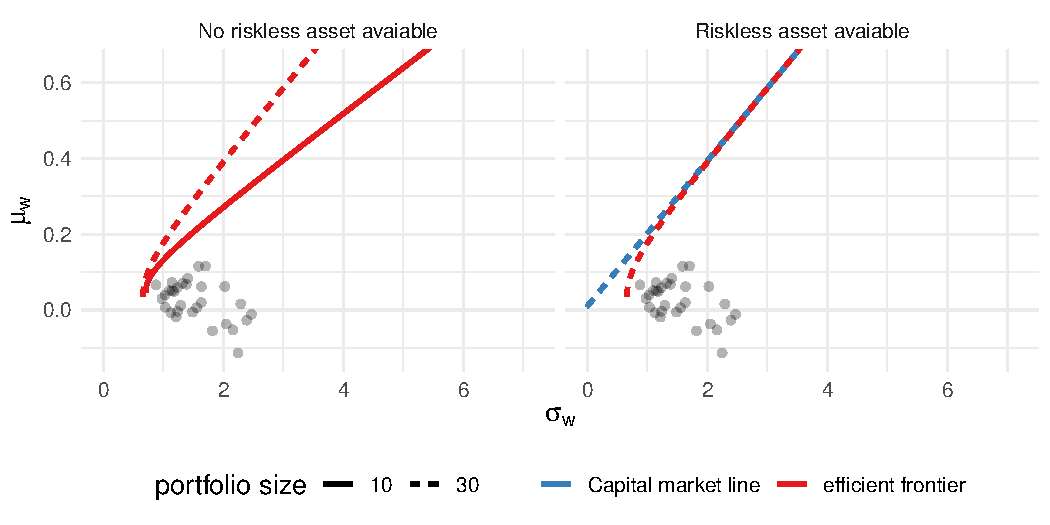
\includegraphics[width=\maxwidth]{figure/mertons_efficient_frontier-1} 

}

\caption[Three different efficient frontiers for different portfolio sizes]{Three different efficient frontiers for different portfolio sizes. The stocks are randomly selected from the S\&P500. The individual means and std. are displayed as points in the background.}\label{fig:mertons_efficient_frontier}
\end{figure}

\end{knitrout}

\section{Relationship between assets and the (inverse) Covariance matrix}\label{subsec:cov_prec_matrix}
%%% ----------------------
The covariance matrix $\bSigma$ and the precision matrix $\bSigma^{-1}$ are fundemental to mean-variance portfolios. In this section we discuss the restrictions we place on the covariance matrix and what the precision matrix actually represent. 

For a vector $\bx$ with finite second moment, the covariance matrix is defined as $\bSigma=\optn{E}((\bx - \bmu)(\bx - \bmu)^\top)$. 
It contains the variances of each individual element of $\bx$ on the diagonal as well as the covariance between every pair of elements on the off-diagonal. 
That is, each diagonal element corresponds to the univariate case where the variance is equal to $\optn{E}((x_i - \mu_i)^2)$. 
A distribution is usually called degenerate or singular if the variance is equal to zero, which holds true in the multivariate context as well. 
If any diagonal element is zero, then the covariance matrix is called singular.  
However, due to the fact that we involve covariances on the off-diagonal we are forced to work with a broader definition.  
Since we work with real matrices in this thesis, we limit the definition accordingly. 
From \citet[ch 14.2]{harville1997matrix} we say that a real symmetric $p\times p$ matrix $\bA$ is called 
\begin{itemize}
	\item positive definite if $\bz^\top \bA \bz > 0$
	\item positive semi-definite if $\bz^\top \bA \bz \geq 0$
\end{itemize}
for all nonzero vectors $\bz \in \mathbbm{R}^p$.
In the multivariate case we need to assert that a quadratic form is (strictly) positive in comparison to the univariate setting where we can observe it through the variance. 
Positive- or semi-positive definite can be quite cumbersome to work with. 
We need to assert that the conditions holds for all vectors $\bz$. 
One necessary condition for a matrix to be positive definite can be derived using the eigenvalues of a matrix and its eigenvalue decomposition. 
As described in \citet[ch. 21]{harville1997matrix}, an eigenvalue (or characteristic root) $\lambda$ is the solution to 
\begin{definition}\label{def:eigenvalue} 
	Let $\bA$ be a $p\times p$ matrix. The characteristic roots (with multiplicity) are given by the solutions to
	\begin{equation*}
		\left|\bA - \lambda \bI\right| = 0
	\end{equation*}
	where $|\cdot|$ is the determinant of a matrix.
\end{definition} 
Let $\lambda_i$, $i=1,2,...,p$, denote the \textit{ordered} eigenvalues of the matrix $\bA$ such that $\lambda_1\geq \lambda_2 \geq ... \geq \lambda_p$.
Given an eigenvalue, the eigenvectors $\bu_i$ are defined by $\bA \bu_i = \lambda_i \bu_i$, $i=1,2,...,p$. 
Let $\boldsymbol{\Lambda} = \operatorname{diag}(\lambda_1, \lambda_2,...,\lambda_p)$ and $\bU= (\bu_1^\top, \bu_2^\top, ..., \bu_p^\top)^\top$. 
Furthermore, we say that $\bB$ is an inverse of $\bA$ if it satisfies $\bB \bA = \bI$, which we usually denote $\bB=\bA^{-1}$.
Using the relation between eigenvalues and their eigenvectors we can derive the eigenvalue decomposition of a symmetric matrix 

\begin{equation}\label{eqn:eigenvalue_decomp}
	\bA = \bU \boldsymbol{\Lambda} \bU^{\top}.
\end{equation}

A necessary condition for a matrix to be positive definite can be directly obtained from the eigenvalue decomposition. 
Let $\bz\in \mathbbm{R}^p$ and $\by := \bU^{\top} \bz \in \mathbbm{R}^p$, then $\bz^\top \bA \bz = \bz^\top \bU \boldsymbol{\Lambda} \bU ^{\top} \bz = \by^\top \boldsymbol{\Lambda} \by = \sum_i^p \lambda_i y_i^2$ which is a second degree polynomial. 
If the eigenvalues are all positive then necessarily the matrix is positive definite. 
If there are some eigenvalues which are zero then the matrix is semi-positive definite. 

In all papers of this thesis we assume that the true covariance matrix is positive definite. 
The assumption has quite a deep economical interpretation.
If one (or more) eigenvalue(s) are zero then there is a possibility to construct a portfolio which does not contain any risk with a potentially positive return. 
An opportunity which should not exist unless the elements of $\bmu$ are all zero.
Assume $\lambda_p=0$, let $\bu_p$ be its eigenvector and set $\bw = \bu_p / \sum_i^p u_{ip}$. The variance of that portfolio is zero since all eigenvectors are orthonormal and its mean is $\bw^\top \bmu$ which can be non-zero unless the elements of $\bmu$ are all zero.
If the true covariance matrix is not positive definite there might exist arbitrage opportunities, e.g. the possibility of making profit without taking any risk.

The eigenvalue decomposition is very useful.
First, it provides a simple way to construct inverses, which is very important for MPT as seen in \eqref{eqn:mean_var_solution}.
We claim that $\bB = \bU \boldsymbol{\Lambda}^{-1} \bU^{\top}$ is a valid inverse which is easy to verify since $\bB \bA = \bU \boldsymbol{\Lambda}^{-1} \bU^{\top} \bU \boldsymbol{\Lambda} \bU^{\top}$. 
To study the inverse we need to study the ionverse of the eigenvalues.
Secondly, it contains a lot of information that might not be available at first glance. 
If $\bA$ is a covariance matrix then it contains variances and covariances, describing relations between random variables. 
The eigenvectors are rotations that try to capture as much variation as possible along its axis.
The eigenvalues is the variation along the eigenvectors axis. 
They describes how the system behaves and not the individual elements and their inverse values describe how the precision matrix behaves.
\textbf{comment on latent factors}

%%%%%% ------------------------------------------------------------------------
\chapter{Statistical models and estimation}\label{ch:estim}
%%%%%% ------------------------------------------------------------------------

To \textit{pratically} use the portfolios described by \eqref{eqn:mean_var_solution} we have to specify $\bmu$ and $\bSigma$.


To state his portfolio allocation problem we first introduce the relevant quantities. In this thesis we never use the asset prices themselves but their a transformation of the relative differences, that is, their simple returns. The simple return is defined as $r_{i,t} := (y_{i,t}-y_{i,t-1})/y_{i,t-1}$ and the log return is then defined as
$
x_{i,t} := \log(r_{i,t} + 1)
$
where $y_{i,t}$ is the price of the $i$th asset at time $t$. We model a portfolio with $p$ assets as $\sum_{i=1}^p w_i x_{i,t} = \bw^\top \bx_t$ where $\bw=(w_1, ..., w_p)$ are the portfolio weights and $\bx_t=(x_{1,t},x_{2,t},..., x_{p,t})$ are the log returns. Notice that this is an approximation. In reality we would want to work with $\sum_{i=1}^p w_i r_{i,t}$ since it is additive in the number of assets. However, logarithmic returns are additive in time which can be desirable. Compounding returns results in simple addition. The difference between the two approaches is very small if the returns are small, which is often true for financial assets. The models we work with in this thesis often rely on the log returns and not the returns. We will omit the time index $t$ to keep the notation tidy unless otherwise stated. 

\begin{itemize}
	\item Multivariate Normal
	\item Wishart and inverse wishart distribution, properties
	\item Matrix variate location and scale. 
\end{itemize}

\begin{definition}
	A random vector $\bx \in \mathbbm{R}^p$ follows a multivariate normal distribution with mean vector $\bmu \in \mathbbm{R}^p$ and positive definite covariance matrix  $\bSigma \in \mathbbm{R}^{p \times\, p}$ if its density is given by 
	\begin{equation}\label{eqn:multi_density}
	\frac{|\bSigma|^{-1/2}}{2\pi} \exp \left\{-\frac{1}{2} \left(\bx - \bmu \right)^\top\bSigma^{-1}\left(\bx - \bmu \right) \right\}
	\end{equation}
	where $|\bB|$ is the determinant of the matrix $\bB$. We usually use the notation $\bx \sim N_p(\bmu, \bSigma)$ to indicate the above.
\end{definition} 

\begin{definition}
	The random matrix $\bS$ of size $p \times p$ follows a $p\times p$ dimensional Wishart distribution with $n$ degrees of freedom, $n > p$, if its density is given by
	\begin{equation}\label{eqn:wishart_density}
	\frac{|\bS|^{(n-p-1)/2} |\bSigma|^{- n/2} }{2^{pn/2} \Gamma_p (n/2) } \exp\left\{-\frac{1}{2} \operatorname{tr}(\bSigma^{-1}\bS)  \right\}
	\end{equation}
	where $ \Gamma_p (\cdot) $ is the multivariate gamma function and $\operatorname{tr}(\cdot)$ is the trace operator, i.e. the sum of the diagonal elements and $\bSigma, \bS$ are both positive definitie. We use the notation $\bS \sim W_p(n, \bSigma)$ to indicate that $\bS$ follows a Wishart distribution with the given parameters.
\end{definition}

\begin{definition}
	A positive definitie random matrix $\bA$ is said to be distributed according to a $p\times p$ dimensional inverse Wishart distribution with $n$ degrees of freedom and positive definitie parameter matrix $\bV$ if its density is given by
	\begin{equation}\label{eqn:inverse_wishart}
	\frac{2^{-(n-p-1)p/2} |\bSigma|^{(n-p-1)/2} }{\Gamma_p ((n-p-1)/2) |\bA|^{n/2}} \exp\left\{ -\frac{1}{2} \bA \bV \right\}, \; n> 2p
	\end{equation}
	which we denote $\bA \sim W^{-1}_p(n, \bV)$ to indicate that $\bV$ follows an Inverse Wishart distribution with the given parameters.
\end{definition}


\begin{lemma}\label{lem:stoc_rep}
	$\bx$ is a $k$ dimensional elliptically contoured distributed random variable with mean $\bmu$ and dispersion matrix $\bSigma$ where $\text{rk} (\bSigma) = p$, if and only if 
	$$
	\bx \stackrel{d}{=} \bmu + r \bV \bu
	$$
	where $r >0$ is a random variable, $\bu$ is a random vector which is uniformly distributed on the sphere, in $\mathbbm{R}^k$, $\bV\bV^\top=\bSigma$, and $r$ and $\bu$ are independent.
\end{lemma}

\section{Estimation - the name of the game}

\begin{itemize}
	\item What are the implications of using $\bS$ instead of $\bSigma$?
	\item why is $\bS$  always an admissible estimator? (MM)
	\item Other types of estimators and why they might be better than $\bS$.
\end{itemize}

\begin{remark}
	Unconditional and conditional covariance estimation. Prediction is very hard and constructing viable models. Are returns predictable? Should we even try?
\end{remark}

\section{Simulations, inverses and why stochastic representations are valuable}
\begin{itemize}
	\item Motivating simulations and the issue with inversions.
	\item Simulation of multi- or matrixvariate distributions can be very computationally consuming.
	\item ...
\end{itemize}
%%%%%% ------------------------------------------------------------------------
\chapter{Higher dimensions or portfolios with many assets}\label{ch:highdim}
%%%%%% ------------------------------------------------------------------------

In the previous chapter we presented different ways of estimating the covariance matrix. Under certain conditions and/or statistical models, the sample covariance matrix inherited certain properties. 
%If we hold $p$ constant and let $n$ grow the sample covariance matrix is consistent. 
If we have a lot of data on the assets that we are trying to invest in then we can most often be certain that we will hold the correct portfolio.
Our estimated portfolio will be consistent, e.g. it estimates the correct object of interest. 
However, if we believe in diversification then $p$ should be big as well. 
It should, in theory, decrease the risk (variance) of the portfolio. 
That is not always the case.
By introducing one new asset to our portfolio of size $p$ we need to estimate the variance and all covariances in the sample covariance matrix. They constitute an additional $p+1$ quantities. 
The sample covariance matrix suffers from the curse of dimensionality. 
In terms of estimation uncertainty, this does not scale well. 

\begin{itemize}
  \item \textbf{state the implications of large dimensions for portfolio theory}, Consistency of $\bS$ but not of $\bS^{-1}$.
	\item Give small example of the different quantities on how they behave
	\item In terms of simulation, this becomes even worse.
\end{itemize}

\section{Random Matrix Theory and Stieltjes transforms}
The subject of Random matrix theory (RMT) has many applications. It was originally developed in the context of statistical physics by \citet{} WIGNER. The theory has developed and is now used in many fields such as combinatorics, computational biology, wireless communication and finance. This section gives a brief introduction and will then cover a small part of the field more indepth, namely high dimensional limits involving the inverse sample covariance matrix and transformations thereof. 





\begin{itemize}
  \item The Marcenko-Pastur (MP) law?
  \item Short on Stieltjes transforms.
	\item Theorem 1 of \citet{rubio2011spectral}.
\end{itemize}


%%%%%% ------------------------------------------------------------------------
\chapter{Summary of Papers}\label{ch:papersummary}
%%%%%% ------------------------------------------------------------------------

The papers presented here are among a total of ... papers produced. These are selected based their common theme.
\section*{Paper 1 - Sampling ...}
The paper investigates a fundemental question in modern portfolio theory. 
What are the implications to using the sample covariance matrix $\bS$ and the sample mean $\bxb$ instead of the true covariance matrix $\bSigma$ and $\bmu$?
The paper does so when returns follow a multivariate normal distribution.


\section*{Paper 2 - Tangency portfolio}
In this paper we investigate the another portfolio which contains a risk-free asset. The return or rate of the risk-free asset is denoted $r_f$. To introduce this option into our portfolio we add the risk-free rate as part of the portfolio $w_0 r_f + \bw^\top \bx$ and optimize over $w_0$ as well. The portfolio is obtained from the quadratic utility function, that is, it originates from the following portfolio allocation 
\begin{align}
  \min_{w_0,\bw} & w_0 r_f + \bw^\top \bmu - \frac{1}{2\gamma} \bw^\top \bSigma \bw \\
  \text{ s.t.} &\; w_0 + \bw^\top \ones_p = 1
\end{align}
However, since $w_0 + \bw^\top \ones=1$ we substitute $w_0=1-\bw^\top \ones$ and solve the unconstrained optimization problem instead. The portfolio has many interesting properties. If there is a risk-free asset we can actually increase the return and decrease the risk of our position in the market. This is most easily explained by the efficient frontier, displayed in Figure \ref{fig:mertons_efficient_frontier}, and what happens with it when the risk-free rate is introduced. In Figure \ref{fig:paper2-summary} we illustrate what happens. Since we have the opportunity to invest in a risk-free asset we can decrease the risk we take in comparison to earlier. If we do not want to take any market risk, then we can place all our cash in a bond with rate $r_f$. Taking any combination between will result in less risk and more return.  
\begin{knitrout}
\definecolor{shadecolor}{rgb}{0.969, 0.969, 0.969}\color{fgcolor}\begin{figure}

{\centering 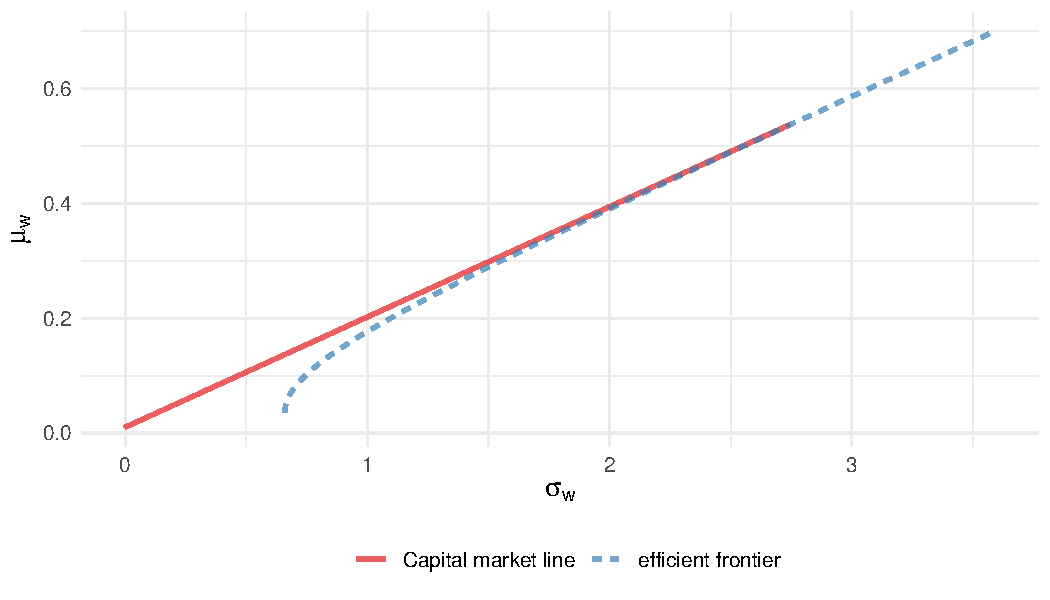
\includegraphics[width=\maxwidth]{figure/paper2summary-1} 

}

\caption[Efficient frontier and the capital market line for 30 (randomly) selected stocks from the S\&P500]{Efficient frontier and the capital market line for 30 (randomly) selected stocks from the S\&P500}\label{fig:paper2summary}
\end{figure}

\end{knitrout}
The paper investigates what the distribution is of the tangency portfolio, or in a more broader context, the capital market line. We use an extension to the multivariate Gaussian Model from Paper 1, the Closed Skew-Normal Matrixvariate Model. This model can include skewness in the asset returns a trait returns usually exhibit (see e.g. \cite{cont2001empirical}). We investigate what implications the model has on the estimated tangency portfolio.
\section*{Paper 3}
This paper deals with the fact that taking limits changes estimates. Assuming that the investor is interested in daily returns then if he/she invest in the GMV portfolio today and wait a week the estimates of the portfolio estimate will have changed.  Rebalancing every day will induce a cost. Assuming that we are ok with rebalancing the portfolio at fixed time points, which could be daily, we develop a reweighting scheme the induced cost. That is, minimize the movement between portfolio reallocations.

This paper continues on to use another model. Although more general, its also 

The paper is accompanied by a R package, available on CRAN. You are free\footnote{or rather encouraged!} to install it by \hlkwd{install.packages}\hlstd{(}\hlstr{"DOSPortfolio"}\hlstd{)}. Below is a short introduction on how to construct the portfolio estimates  
\begin{knitrout}
\definecolor{shadecolor}{rgb}{0.969, 0.969, 0.969}\color{fgcolor}\begin{kframe}
\begin{alltt}
\hlstd{df} \hlkwb{<-} \hlkwd{read_csv}\hlstd{(}\hlstr{"../data/returns.csv"}\hlstd{)}
\hlkwd{library}\hlstd{(DOSPortfolio)}
\hlkwd{set.seed}\hlstd{(}\hlnum{1234}\hlstd{)}
\hlstd{p} \hlkwb{<-} \hlnum{350}\hlstd{; n} \hlkwb{<-} \hlnum{400}
\hlcom{# Sample p assets}
\hlstd{asset_cols} \hlkwb{<-} \hlkwd{sample}\hlstd{(}\hlnum{2}\hlopt{:}\hlkwd{ncol}\hlstd{(df),} \hlkwc{size} \hlstd{= p)}
\hlcom{# specify reallocation points}
\hlstd{reallocation_points} \hlkwb{<-} \hlkwd{seq}\hlstd{(n,} \hlkwd{nrow}\hlstd{(df),} \hlkwc{by}\hlstd{=n)}
\hlcom{# estimate portfolio weights}
\hlstd{dos_weights} \hlkwb{<-} \hlstd{df} \hlopt
  \hlkwd{select}\hlstd{(}\hlkwd{all_of}\hlstd{(asset_cols),} \hlopt{-}\hlstd{date)} \hlopt
  \hlkwd{DOSPortfolio}\hlstd{(.,}
               \hlkwc{reallocation_points} \hlstd{= reallocation_points,}
               \hlkwc{target_portfolio} \hlstd{=} \hlkwd{rep}\hlstd{(}\hlnum{1}\hlstd{,} \hlkwd{ncol}\hlstd{(.))}\hlopt{/}\hlkwd{ncol}\hlstd{(.),}
               \hlkwc{shrinkage_type} \hlstd{=} \hlstr{"overlapping"}\hlstd{)}
\end{alltt}
\end{kframe}
\end{knitrout}



% In Figure  \ref{fig:examplePackage} we can see the wealth and how it develops throughout a little more than 6 years. Although the GMV portfolio is a poor choice in this scenario indicate that the DOSPortfolio is better in terms of welath
\section*{Paper 4}
Double shrinkage?
%%%%%% ------------------------------------------------------------------------
\chapter{Future research}\label{ch:future}
%%%%%% ------------------------------------------------------------------------

There are many possible extensions and future projects to the thesis at hand.

\begin{itemize}
	\item Are shrinkage intensities for the sample covariance matrix optimal for the precision or MPT problem? 
	\item One of the most interesting issues of the elliptical distribution and its inverse sample dispersion matrix. What are the moments of $(\mathbf{Z} \mathbf{R} \mathbf{Z}^\top)^{-1}$?
	\item There are different ways of incorporating estimation uncertainty, one solution is robust optimization. Are there connections to be made? Is robust optimization just Emperical Bayes?
	\item Sequential reweighting extension to Paper 3. When should we reweight?
	\item Higher dimensions, other estimators, hard shrinkage.
	\item BEKK models are usually hard to fit and use for MPT. Their forecasts are not always positive definite. The first issue is simple to cope with if one can formulate the models as Recurrent Neural Networks and use the efficient deep-learning libraries Torch or Tensorflow. By doing so, one would also get the possibility to develop new models by constructing new layers to the networks. It would also be easier to integrate different sources of information in the models.
\end{itemize}

Although not part of this Phd thesis - Flipped classroom and online learning tools.
\bibliography{references}

%%%%%%%%%%%%%%%%%%%%%%%%%%%%%%%%%%%%%%%%%%
% Insert papers here
%%%%%%%%%%%%%%%%%%%%%%%%%%%%%%%%%%%%%%%%%%

\end{document}
